\textbf{Questão 1}

Neste trabalho, você irá ajustar e avaliar três modelos diferentes em um conjunto de dados com três features:

\begin{enumerate}
    \item \textbf{GaussI}: Um modelo de mistura de Gaussianas (GMM) com uma Gaussiana por classe, onde as matrizes de covariância são todas iguais à matriz identidade, i.e., \( p(x|y = c) = N(x|\mu_c, I) \).
    
    \item \textbf{GaussX}: Um modelo de mistura de Gaussianas (GMM) com uma Gaussiana por classe, sem restrições nas matrizes de covariância, i.e., \( p(x|y = c) = N(x|\mu_c, \Sigma_c) \).
    
    \item \textbf{LogReg}: Um modelo de regressão logística com características lineares e quadráticas, i.e., função polinomial de grau 2.
\end{enumerate}

A questão inclui dois conjuntos de dados: um conjunto de treino e um conjunto de teste. Cada amostra possui três features. Siga os passos a seguir para cada modelo:

\begin{enumerate}
    \item Calcule a log-likelihood, de forma literal para cada modelo (explique como calcular os parâmetros de cada).
    \begin{tcolorbox}[title=Resposta:]
        
        \begin{itemize}
            \item \textbf{Modelo GaussI: Mistura de Gaussianas com Matriz Identidade}
        
            No modelo GaussI, todas as classes \( c \) são representadas por uma gaussiana multivariada com média \( \mu_c \) e matriz de covariância igual à identidade \( I \). Sendo uma mistura de gaussianas, o peso \( \pi_c \) da classe \( c \) representa a proporção de amostras pertencentes àquela classe na mistura. A função de densidade de probabilidade para uma amostra \( x \) é dada por:
            \[
            p(x) = \sum_{c} \pi_c \, N(x | \mu_c, I) = \sum_{c} \pi_c \, \frac{1}{(2\pi)^{d/2}} \exp \left( -\frac{1}{2} (x - \mu_c)^T (x - \mu_c) \right)
            \]

            \textbf{Cálculo da Log-Likelihood:}  
            Dada uma amostra \( X = \{x_1, x_2, \dots, x_n\} \), a log-likelihood do modelo é:
            \[
            \mathcal{L}(\theta | X) = \sum_{i=1}^n \log \left( \sum_{c} \pi_c \, p(x_i | y=c) \right)
            \]
            Substituindo \( p(x_i | y=c) \):
            \[
            \mathcal{L}(\theta | X) = \sum_{i=1}^n \log \left( \sum_{c} \pi_c \, \frac{1}{(2\pi)^{d/2}} \exp \left( -\frac{1}{2} (x_i - \mu_c)^T (x_i - \mu_c) \right) \right)
            \]
        
            \textbf{Cálculo dos Parâmetros:}  
            Utilizando o Maximum Likelihood Estimation (MLE), os parâmetros do modelo são ajustados derivando-se a log-likelihood em relação a \( \mu_c \) e \( \pi_c \) e igualando a zero.
            Para cada classe \( c \):
            \begin{itemize}
                \item A média \( \mu_c \) é estimada pela média das amostras de treino da classe \( c \):
                \[
                \mu_c = \frac{1}{n_c} \sum_{i=1}^{n_c} x_i
                \]
                \item O peso \( \pi_c \) é estimado como a proporção de amostras da classe \( c \) no conjunto de treino:
                \[
                \pi_c = \frac{n_c}{n}
                \]
                onde \( n_c \) é o número de amostras da classe \( c \) e \( n \) é o total de amostras.
            \end{itemize}

           

        \end{itemize}

        \end{tcolorbox}

        \begin{tcolorbox}[title=Resposta (continuação):]

        \begin{itemize}

            \item \textbf{Modelo GaussX: Mistura de Gaussianas sem Restrições na Covariância}
        
            Neste modelo, cada classe \( c \) é representada por uma gaussiana com média \( \mu_c \) e matriz de covariância \( \Sigma_c \). Assim, a função de densidade de probabilidade é:
            \[
            p(x) = \sum_{c} \pi_c \, N(x | \mu_c, \Sigma_c) = \sum_{c} \pi_c \, \frac{1}{(2\pi)^{d/2} |\Sigma_c|^{1/2}} \exp \left( -\frac{1}{2} (x - \mu_c)^T \Sigma_c^{-1} (x - \mu_c) \right)
            \]

            \textbf{Cálculo da Log-Likelihood:}  
            A log-likelihood para o modelo é:
            \[
            \mathcal{L}(\theta | X) = \sum_{i=1}^n \log \left( \sum_{c} \pi_c \, p(x_i | y=c) \right)
            \]
            Substituindo \( p(x_i | y=c) \):
            \[
            \mathcal{L}(\theta | X) = \sum_{i=1}^n \log \left( \sum_{c} \pi_c \, \frac{1}{(2\pi)^{d/2} |\Sigma_c|^{1/2}} \exp \left( -\frac{1}{2} (x_i - \mu_c)^T \Sigma_c^{-1} (x_i - \mu_c) \right) \right)
            \]

            \textbf{Cálculo dos Parâmetros:}  
            Utilizando também o MLE, os parâmetros do modelo são ajustados derivando-se a log-likelihood em relação a \( \mu_c \), \( \Sigma_c \) e \( \pi_c \) e igualando a zero.
            Para cada classe \( c \):
            \begin{itemize}
                \item A média \( \mu_c \) é calculada pela média das amostras de treino da classe \( c \):
                \[
                \mu_c = \frac{1}{n_c} \sum_{i=1}^{n_c} x_i
                \]
                \item A matriz de covariância \( \Sigma_c \) é estimada por:
                \[
                \Sigma_c = \frac{1}{n_c} \sum_{i=1}^{n_c} (x_i - \mu_c)(x_i - \mu_c)^T
                \]
                \item O peso \( \pi_c \) é dado pela proporção de amostras da classe \( c \):
                \[
                \pi_c = \frac{n_c}{n}
                \]
            \end{itemize}

        
        

        \end{itemize}
        
        \end{tcolorbox}

        \begin{tcolorbox}[title=Resposta (continuação):]

            \begin{itemize}
        
                \item \textbf{Modelo LogReg: Regressão Logística com Features Lineares e Quadráticas}
            
                Para o modelo de regressão logística, definimos uma função de probabilidade que modela a probabilidade de \( y = 1 \) ou \( y = 2 \) como uma função logística das features lineares e quadráticas.
            
                A probabilidade de uma amostra \( x \) pertencer à classe \( y = 1 \) é:
                \[
                p(y=1|x) = \sigma(w^T x + w_q^T x^2 + b)
                \]
                onde:
                \begin{itemize}
                    \item \( \sigma(z) = \frac{1}{1 + e^{-z}} \) é a função sigmoide,
                    \item \( w \) e \( w_q \) são vetores de pesos para as features lineares e quadráticas, respectivamente,
                    \item \( b \) é o bias (intercepto).
                \end{itemize}
            
                \textbf{Cálculo da Log-Likelihood:}  
                A log-likelihood para o modelo de regressão logística com \( n \) amostras é:
                \[
                \begin{aligned}
                    \mathcal{L}(\theta | X, y) = & \sum_{i=1}^n \left( \delta_{y_i,1} \log \sigma(w^\top x_i + w_q^\top x_i^2 + b) \right. \\ 
                    & \left. + \delta_{y_i,2} \log (1 - \sigma(w^\top x_i + w_q^\top x_i^2 + b)) \right)
                \end{aligned}
                \]
                onde \( \delta_{y_i,1} \) e \( \delta_{y_i,2} \) são funções indicadoras que valem 1 quando \( y_i = 1 \) e \( y_i = 2 \), respectivamente, e 0 caso contrário.
    
            
                \textbf{Cálculo dos Parâmetros:}  
                Os parâmetros \( w \), \( w_q \) e \( b \) são obtidos por maximização da log-likelihood, que geralmente é resolvida através de métodos de otimização numérica, como gradiente descendente ou variantes (ex.: método de Newton-Raphson).
            
            \end{itemize}

        \end{tcolorbox}

        
    \item Para cada modelo (GaussI, GaussX e LogReg), obtenha os parâmetros usando o conjunto de treino.
    \begin{tcolorbox}[title=Resposta:]
        
        \begin{itemize}
            \item \textbf{Modelo GaussI}: 
            \begin{itemize}
                \item \textbf{Média \( \mu_c \)}: Calculamos a média \( \mu_c \) para cada classe \( c \) somando todas as amostras da classe e dividindo pelo número total de amostras dessa classe:
                \[
                \mu_c = \frac{1}{n_c} \sum_{i=1}^{n_c} x_i
                \]
                onde \( n_c \) é o número de amostras da classe \( c \).
                
                \item \textbf{Peso \( \pi_c \)}: O peso \( \pi_c \) da mistura para a classe \( c \) é a proporção de amostras da classe \( c \) no conjunto de treino:
                \[
                \pi_c = \frac{n_c}{n}
                \]
                onde \( n \) é o total de amostras.
                
                \item \textbf{Covariância}: A matriz de covariância é a identidade \( I \), sendo fixa para todas as classes.
            \end{itemize}
        
            \item \textbf{Modelo GaussX}: 
            \begin{itemize}
                \item \textbf{Média \( \mu_c \)}: Calculamos a média \( \mu_c \) da mesma forma que no GaussI.
                
                \item \textbf{Peso \( \pi_c \)}: O peso \( \pi_c \) é estimado da mesma forma que no GaussI
        
                \item \textbf{Covariância \( \Sigma_c \)}: Estimamos a matriz de covariância \( \Sigma_c \) para cada classe \( c \) como:
                \[
                \Sigma_c = \frac{1}{n_c} \sum_{i=1}^{n_c} (x_i - \mu_c)(x_i - \mu_c)^T
                \]
            \end{itemize}
        
            \item \textbf{Modelo LogReg}: 
            \begin{itemize}
                \item Ajustaremos os parâmetros \( w \), \( w_q \), e \( b \) para maximizar a log-likelihood do modelo no conjunto de treino, onde as classes são \( y = 1 \) e \( y = 2 \). Para isso, utilizamos métodos de otimização, como o método quasi-Newton Broyden-Fletcher-Goldfarb-Shanno (BFGS).
            \end{itemize}
        \end{itemize}
        
        \end{tcolorbox}

        \begin{tcolorbox}[title=Resposta (continuação):]
            \begin{itemize}
                
                \item \textbf{GaussI}
                    Média classe 1: [9.87137785, 10.10450844, 10.03867547] \\
                    Média classe 2: [5.00268659 4.96179356 5.02277374] \\
                    Matriz de covariância (identidade): 
                    \[
                    \begin{bmatrix}
                        1.0 & 0.0 & 0.0 \\
                        0.0 & 1.0 & 0.0 \\
                        0.0 & 0.0 & 1.0 \\
                    \end{bmatrix}
                    \]
                    Peso da classe 1: 0.7142857142857143 \\
                    Peso da classe 2: 0.2857142857142857

                
                \item \textbf{GaussX}
                    Média classe 1: [9.87137785, 10.10450844, 10.03867547] \\
                    Covariância classe 1:
                    \[
                    \begin{bmatrix}
                        1.06499084 & 0.23280792 & 0.0827585 \\
                        0.23280792 & 0.97380852 & 0.31446581 \\
                        0.0827585  & 0.31446581 & 1.11015715 \\
                    \end{bmatrix}
                    \]
                    Média classe 2: [5.00268659, 4.96179356, 5.02277374] \\
                    Covariância classe 2:
                    \[
                    \begin{bmatrix}
                        1.01006542 & -0.1147753 & 0.03187256 \\
                        -0.1147753 & 0.90176172 & 0.18048772 \\
                        0.03187256 & 0.18048772 & 0.92142339 \\
                    \end{bmatrix}
                    \]
                    Peso da classe 1: 0.7142857142857143 \\
                    Peso da classe 2: 0.2857142857142857
                
                
                \item \textbf{LogReg}
                    Coeficientes (w): [-369.8030754, -419.75537071, -308.97310576] \\
                    Intercepto (b): 8620.82826196496

            \end{itemize}
        
        \end{tcolorbox}

    
        
    \item Para cada modelo (GaussI, GaussX e LogReg), calcule a log-likelihood usando o conjunto de teste e os parâmetros obtidos.
    \begin{tcolorbox}[title=Resposta:]
        Foram utilizadas, em um código Python, as fórmulas de log-likelihood deduzidas no item 1 para calcular o valor da log-likelihood de cada modelo no conjunto de dados de treinamento (não foi possível utilizar o conjunto de teste, pois o mesmo está sem labels). Abaixo estão os resultados obtidos para cada modelo:
        
        \begin{itemize}
            \item \textbf{Log-Likelihood GaussI}: -3416.1258637693318
            \item \textbf{Log-Likelihood GaussX}: -3370.0326509880647
            \item \textbf{Log-Likelihood LogReg}: -6.263139306057298e-07
        \end{itemize}
    \end{tcolorbox}
    
    \item Avalie o desempenho de cada modelo usando o conjunto de teste e compare os resultados. Discuta qual modelo apresentou o melhor desempenho e tente dar a sua explicação sobre o motivo.
    
    \begin{tcolorbox}[title=Resposta:]
        Como não foi possível utilizar o conjunto de teste, não foi possível avaliar o desempenho dos modelos. No entanto, podemos comparar os valores de log-likelihood obtidos no conjunto de treinamento. O modelo de regressão logística apresentou o maior valor de log-likelihood, indicando que ele se ajustou melhor aos dados de treinamento.

        As matrizes de confusão e as acurácias obtidos no conjunto de treinamento para cada modelo podem ser visualizados na Figura \ref{fig:confusion_matrices}.
    \end{tcolorbox}

    \begin{figure}[H]
        \centering
        \begin{subfigure}[b]{0.3\textwidth}
            \centering
            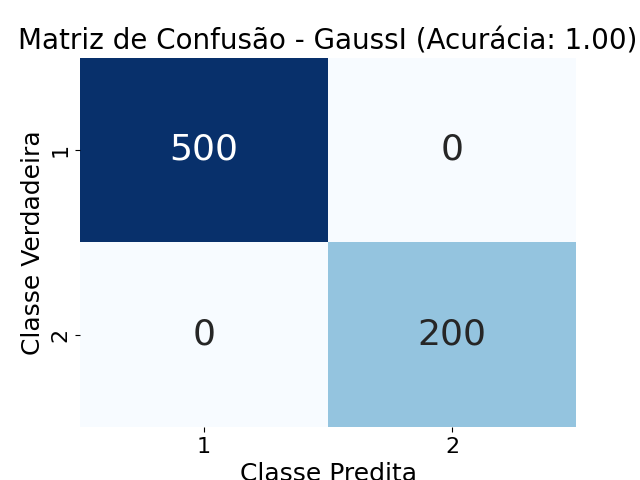
\includegraphics[width=\textwidth]{fig/GaussI.png}
            \caption{Matriz de confusão do modelo GaussI.}
            \label{fig:confusion_matrix_gaussi}
        \end{subfigure}
        \hfill
        \begin{subfigure}[b]{0.3\textwidth}
            \centering
            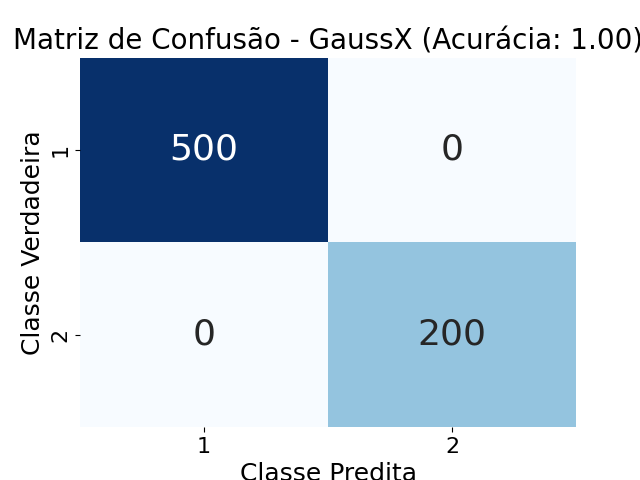
\includegraphics[width=\textwidth]{fig/GaussX.png}
            \caption{Matriz de confusão do modelo GaussX.}
            \label{fig:confusion_matrix_gaussx}
        \end{subfigure}
        \hfill
        \begin{subfigure}[b]{0.3\textwidth}
            \centering
            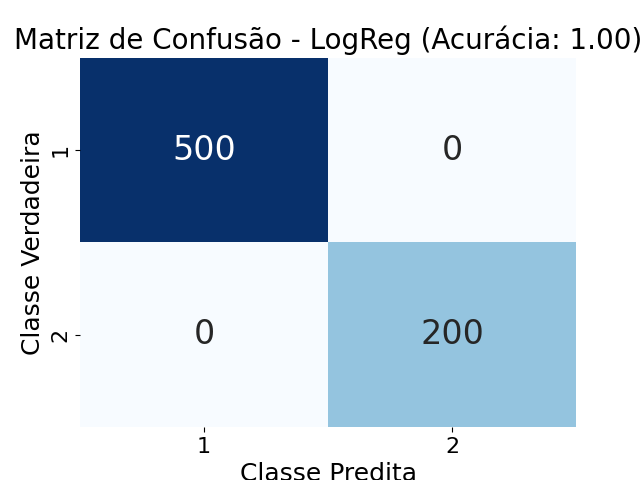
\includegraphics[width=\textwidth]{fig/LogReg.png}
            \caption{Matriz de confusão do modelo LogReg.}
            \label{fig:confusion_matrix_logreg}
        \end{subfigure}
        \caption{Matrizes de confusão dos modelos GaussI, GaussX e LogReg.}
        \label{fig:confusion_matrices}
    \end{figure}

\end{enumerate}
